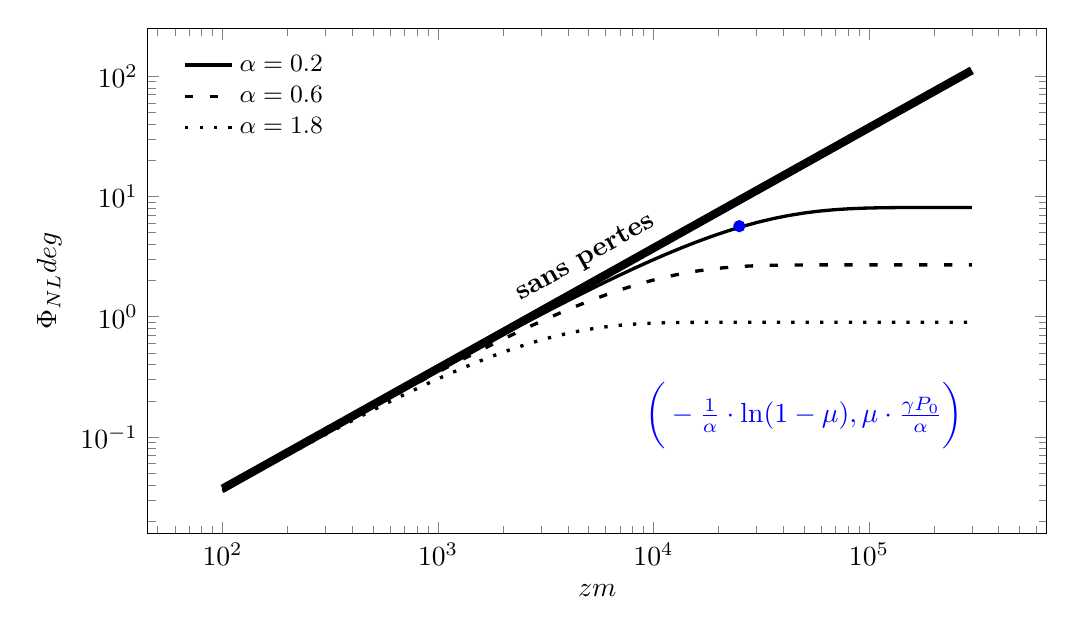
\begin{tikzpicture}
    \begin{loglogaxis}[
        height=8cm,
        width=13cm,
        ylabel={$\Phi_{\text{NL}}\myunit{deg}$},
        xlabel={$z\myunit{m}$},
        legend entries={$\alpha=0.2$,$\alpha=0.6$,$\alpha=1.8$},
        legend style={draw = none, font=\small},
        legend pos=north west,
        grid=none
    ]
        \addplot [
            black,
            domain      = 100:3e5,
            samples     = 50,
            line width  = 1.2pt
        ]
        {0.0013*0.005*1/0.000046*(1-exp(-0.000046*x))*180/3.141592653589};

        \addplot [
            black,
            domain  = 100:3e5,
            samples = 100,
            loosely dashed,
            line width = 1.2pt
        ]
        {0.0013*0.005*1/0.000138*(1-exp(-0.000138*x))*180/3.141592653589};

        \addplot [
            black,
            domain  = 100:3e5,
            samples = 100,
            loosely dotted,
            line width = 1.2pt
        ]
        {0.0013*0.005*1/0.000414*(1-exp(-0.000414*x))*180/3.141592653589};

        \addplot [
            black,
            domain      = 100:3e5,
            samples     = 50,
            line width  = 3pt
        ]
        {0.0013*0.005*1*x*180/3.141592653589} 
        node[sloped,midway,above]{\textbf{sans pertes}};

        \addplot [only marks, color=blue] coordinates {
            (25000, 0.0013*0.005/0.000046052*0.7*180/3.141592653589)
        };

        \node[blue] at (axis cs: 5e4,1.5e-1)
        {$\bigg(-\frac{1}{\alpha} \cdot \ln(1-\mu), \mu \cdot \frac{\gamma P_0}{\alpha}\bigg)$};

    \end{loglogaxis}
\end{tikzpicture}

